%
% This is a borrowed LaTeX template file for lecture notes for CS267,
% Applications of Parallel Computing, UCBerkeley EECS Department.
%

\documentclass{article}
\usepackage{titlesec}
%\setlength{\oddsidemargin}{0.25 in}
%\setlength{\evensidemargin}{-0.25 in}
\setlength{\oddsidemargin}{0 in}
\setlength{\evensidemargin}{0 in}
\setlength{\topmargin}{-0.6 in}
\setlength{\textwidth}{6.5 in}
\setlength{\textheight}{8.5 in}
\setlength{\headsep}{0.75 in}
\setlength{\parindent}{0 in}
\setlength{\parskip}{0.1 in}


%
% ADD PACKAGES here:
%

\usepackage{amssymb}	% Already loads amsfonts
\usepackage{amsthm}
\usepackage{graphicx}
\usepackage{mathtools}	% Already loads amsmath
\usepackage{hyperref}
\usepackage{enumitem}
\usepackage{clrscode3e}  % for typesetting pseudocode
\usepackage{ulem}
\usepackage[usenames,dvipsnames]{xcolor}
\usepackage{multicol}


% Tikz and setup
\usepackage{tikz}
\usepackage{tikz-cd}
\usetikzlibrary{intersections, angles, quotes, calc, positioning}
\usetikzlibrary{arrows.meta}
\usepackage{pgfplots}
\pgfplotsset{compat=1.13}


\tikzset{
    force/.style={thick, {Circle[length=2pt]}-stealth, shorten <=-1pt}
}

%
% The following commands set up the lecnum (lecture number)
% counter and make various numbering schemes work relative
% to the lecture number.
%
\newcounter{lecnum}
\renewcommand{\thepage}{\thelecnum-\arabic{page}}
\renewcommand{\thesection}{\thelecnum.\arabic{section}}
\renewcommand{\theequation}{\thelecnum.\arabic{equation}}
\renewcommand{\thefigure}{\thelecnum.\arabic{figure}}
\renewcommand{\thetable}{\thelecnum.\arabic{table}}

%
% The following macro is used to generate the header.
%
\newcommand{\lecture}[5]{
   \pagestyle{myheadings}
   \thispagestyle{plain}
   \newpage
   \setcounter{lecnum}{#2}
   \setcounter{page}{1}
   \noindent
   \begin{center}
   \framebox{
      \vbox{\vspace{2mm}
    \hbox to 6.28in { {\bf #1
	\hfill} }
       \vspace{4mm}
       \hbox to 6.28in { {\Large \hfill Lecture #2: #3  \hfill} }
       \vspace{2mm}
       \hbox to 6.28in { {\it Lecturer: #4 \hfill Scribe: #5} }
      \vspace{2mm}}
   }
   \end{center}
   \markboth{Lecture #2: #3}{Lecture #2: #3}
   \vspace*{4mm}
}
\renewcommand{\cite}[1]{[#1]}
\def\beginrefs{\begin{list}%
        {[\arabic{equation}]}{\usecounter{equation}
         \setlength{\leftmargin}{2.0truecm}\setlength{\labelsep}{0.4truecm}%
         \setlength{\labelwidth}{1.6truecm}}}
\def\endrefs{\end{list}}
\def\bibentry#1{\item[\hbox{[#1]}]}

\newcommand{\fig}[3]{
			\vspace{#2}
			\begin{center}
			Figure \thelecnum.#1:~#3
			\end{center}
	}

% Colored theorem styles
\makeatother
\usepackage{thmtools}
\usepackage[framemethod=TikZ]{mdframed}
\mdfsetup{skipabove=1em,skipbelow=1em}

\declaretheoremstyle[
    headfont=\bfseries\sffamily\color{ForestGreen!70!black}, bodyfont=\normalfont,
    mdframed={
        linewidth=2pt,
        rightline=false, topline=false, bottomline=false,
        linecolor=ForestGreen, backgroundcolor=ForestGreen!5,
    },
    spaceabove=8pt
]{thmgreenbox}

\declaretheoremstyle[
    headfont=\bfseries\sffamily\color{NavyBlue!70!black}, bodyfont=\normalfont,
    mdframed={
        linewidth=2pt,
        rightline=false, topline=false, bottomline=false,
        linecolor=NavyBlue, backgroundcolor=NavyBlue!5,
    },
    spaceabove=8pt
]{thmbluebox}

\declaretheoremstyle[
    headfont=\bfseries\sffamily\color{NavyBlue!70!black}, bodyfont=\normalfont,
    mdframed={
        linewidth=2pt,
        rightline=false, topline=false, bottomline=false,
        linecolor=NavyBlue
    },
    spaceabove=8pt
]{thmblueline}

\declaretheoremstyle[
    headfont=\bfseries\sffamily\color{RawSienna!70!black}, bodyfont=\normalfont,
    mdframed={
        linewidth=2pt,
        rightline=false, topline=false, bottomline=false,
        linecolor=RawSienna, backgroundcolor=RawSienna!5,
    },
    spaceabove=8pt
]{thmredbox}

\declaretheoremstyle[
    headfont=\bfseries\sffamily\color{RawSienna!70!black}, bodyfont=\normalfont,
    numbered=no,
    mdframed={
        linewidth=2pt,
        rightline=false, topline=false, bottomline=false,
        linecolor=RawSienna, backgroundcolor=RawSienna!1,
    },
    qed=\qedsymbol,
    spaceabove=8pt
]{thmproofbox}

\declaretheoremstyle[
    headfont=\bfseries\sffamily\color{NavyBlue!70!black}, bodyfont=\normalfont,
    numbered=no,
    mdframed={
        linewidth=2pt,
        rightline=false, topline=false, bottomline=false,
        linecolor=NavyBlue, backgroundcolor=NavyBlue!1,
    },
    spaceabove=8pt
]{thmexplanationbox}

% Use these for theorems, lemmas, proofs, etc.
\theoremstyle{definition}
\declaretheorem[style=thmgreenbox, name=Definition, numberwithin=lecnum]{definition}
\declaretheorem[style=thmbluebox, numbered=no, name=Example]{example}
\declaretheorem[style=thmredbox, name=Theorem, numberwithin=lecnum]{theorem}
\declaretheorem[style=thmredbox, name=Proposition, sibling=theorem]{proposition}
\declaretheorem[style=thmredbox, name=Lemma, sibling=theorem]{lemma}
\declaretheorem[style=thmredbox, name=Corollary, sibling=theorem]{corollary}
% \newtheorem{theorem}{Theorem}[lecnum]
% \newtheorem{lemma}[theorem]{Lemma}
% \newtheorem{claim}[theorem]{Claim}
% \newtheorem{corollary}[theorem]{Corollary}
% \newtheorem{definition}[theorem]{Definition}
\declaretheorem[style=thmblueline, numbered=no, name=Remark]{remark}
\renewenvironment{proof}{{\bf \textit{Proof.}}}{\hfill\rule{2mm}{2mm}}
\makeatletter


% **** IF YOU WANT TO DEFINE ADDITIONAL MACROS FOR YOURSELF, PUT THEM HERE:

\renewcommand\Pr{\mathbb{P}}
\newcommand\Ex{\mathbb{E}}

\newcommand\N{\mathbb{N}}
\newcommand\Z{\mathbb{Z}}
\newcommand\Q{\mathbb{Q}}
\newcommand\R{\mathbb{R}}
\newcommand\C{\mathbb{C}}
\newcommand\F{\mathbb{F}}

\DeclarePairedDelimiter\ceil{\lceil}{\rceil}
\DeclarePairedDelimiter\floor{\lfloor}{\rfloor}
\DeclarePairedDelimiter\anglebrac{\langle}{\rangle}

\begin{document}
\lecture{MAT344 Intro to Combinatorics}{11}{Dilworth's Theorem}{Keegan Dasilva Barbosa}{Kevin Gao}

\section{Poset}

\subsection{Dilworth's Theorem}

\begin{theorem}[Dilworth's Theorem]
    Let $\mathbb{P} = (X,P)$ be a poset with width $w$. There is a partition of $X$ into $w$ chains $C_1,\ldots,C_w$. Moreover, this partition is optimal and it is not possible to cover $\mathbb{P}$ with fewer than $w$ chains.
\end{theorem}

There is also a dual version of Dilworth's theorem.

\begin{theorem}[Dilworth's Theorem (dual)]
    Let $\mathbb{P} = (X,P)$ be a poset with height $h$. There is a partition of $X$ into $h$ antichains $A_1,\ldots,A_h$. Moreover, this partition is optimal and it is not possible to cover $h$ with feweer than $h$ antichains.
\end{theorem}

Assuming the existence of such partition as described in Dilworth's theorem, we first prove optimality.

\begin{proof} (of optimality)
    \hfill

    Let $\mathbb{P} = (X,P)$ be a poset with width $w$. By way of contradiction, suppose that $X$ can be partitioned into $k$ disjoint chains $C_1,\ldots, C_k$ such that $k < w$. Take an antichaim $A$ of size $w$ and consider a map $f:\; A \to \{1,\ldots,k\}$ such that $f(x) = i \iff x \in C_i$ ($f$ outputs the index of the chain containing $x$). However, by Pigeonhole Principle, there is some $C_i$ containing at least two distinct members of $A$ and hence are comparable. This is a contradiction to the assertion that $A$ is an antichain.
\end{proof}

Next, we prove the existence of such optimal partition using induction on $|X|$.

\begin{proof} (of existence)
    \hfill

    \textbf{Base Case}: If $|X| = 1$, the poset contains exactly one element is the one point linear (total) order, so $X$ is a chain itself and we are done.

    \textbf{Inductive Step}: Take a poset $\mathbb{P} = (X,P)$ with width $w$ and height $h$. Assume that Dilworth's theorem holds for all posets with cardinality $k < |X|$.

    Let $C = \{x_1,\ldots,x_h\}$ be a maximal chain in $\mathbb{P}$ and consider the subposet $\mathbb{Q} = (X \setminus C,\, P \cap (X \setminus C)^2)$. Without loss of generality, suppose $x_1 <_{\mathbb{P}} <_{\mathbb{P}} \cdots <_{\mathbb{P}} x_h$. Note that $\mathsf{width}(\mathbb{Q}) \leq \mathsf{width}(\mathbb{P})$.

    Case 1: $\mathsf{width}(\mathbb{Q}) < \mathsf{width}(\mathbb{P})$. Then, $\mathsf{width}(\mathbb{Q}) = w-1$ because we only removed one chain to get from $\mathbb{P}$ to $\mathbb{Q}$ and if the width of $\mathbb{Q}$ is smaller than $w-1$, this would mean that some pair of elements in $C$ is not comparable, which would lead to a contradiction. Apply the induction hypothesis to $\mathbb{Q}$ to cover it with $w-1$ chains $C_1, \ldots, C_{w-1}$. Then, adding back $C$ gives us $C_1,\ldots,C_{w-1},C$, which is a cover of $\mathbb{P}$ with $w$ chains.

    Case 2: $\mathsf{width}(\mathbb{Q}) = \mathsf{width}(\mathbb{P})$. Then, there exists an antichain $A = \{a_1,\ldots,a_w\}$ of size $w$ in $\mathbb{Q}$. Let
    $$
    P^- = \{ x \in P \mid \exists i.\,x \leq_{\mathbb{P}} a_i \}
    $$
    $$
    P^+ = \{ x \in P \mid \exists i.\, x \geq_{\mathbb{P}} a_i \}
    $$
    Pictorially, $P^+$ is the set of all elements larger than some $a_i$ under $\leq_{\mathbb{P}}$ and $P^-$ is the set of all elements smaller than some $a_i$ under $\leq_{\mathbb{P}}$.

    \begin{figure}[htbp]
        \centering
        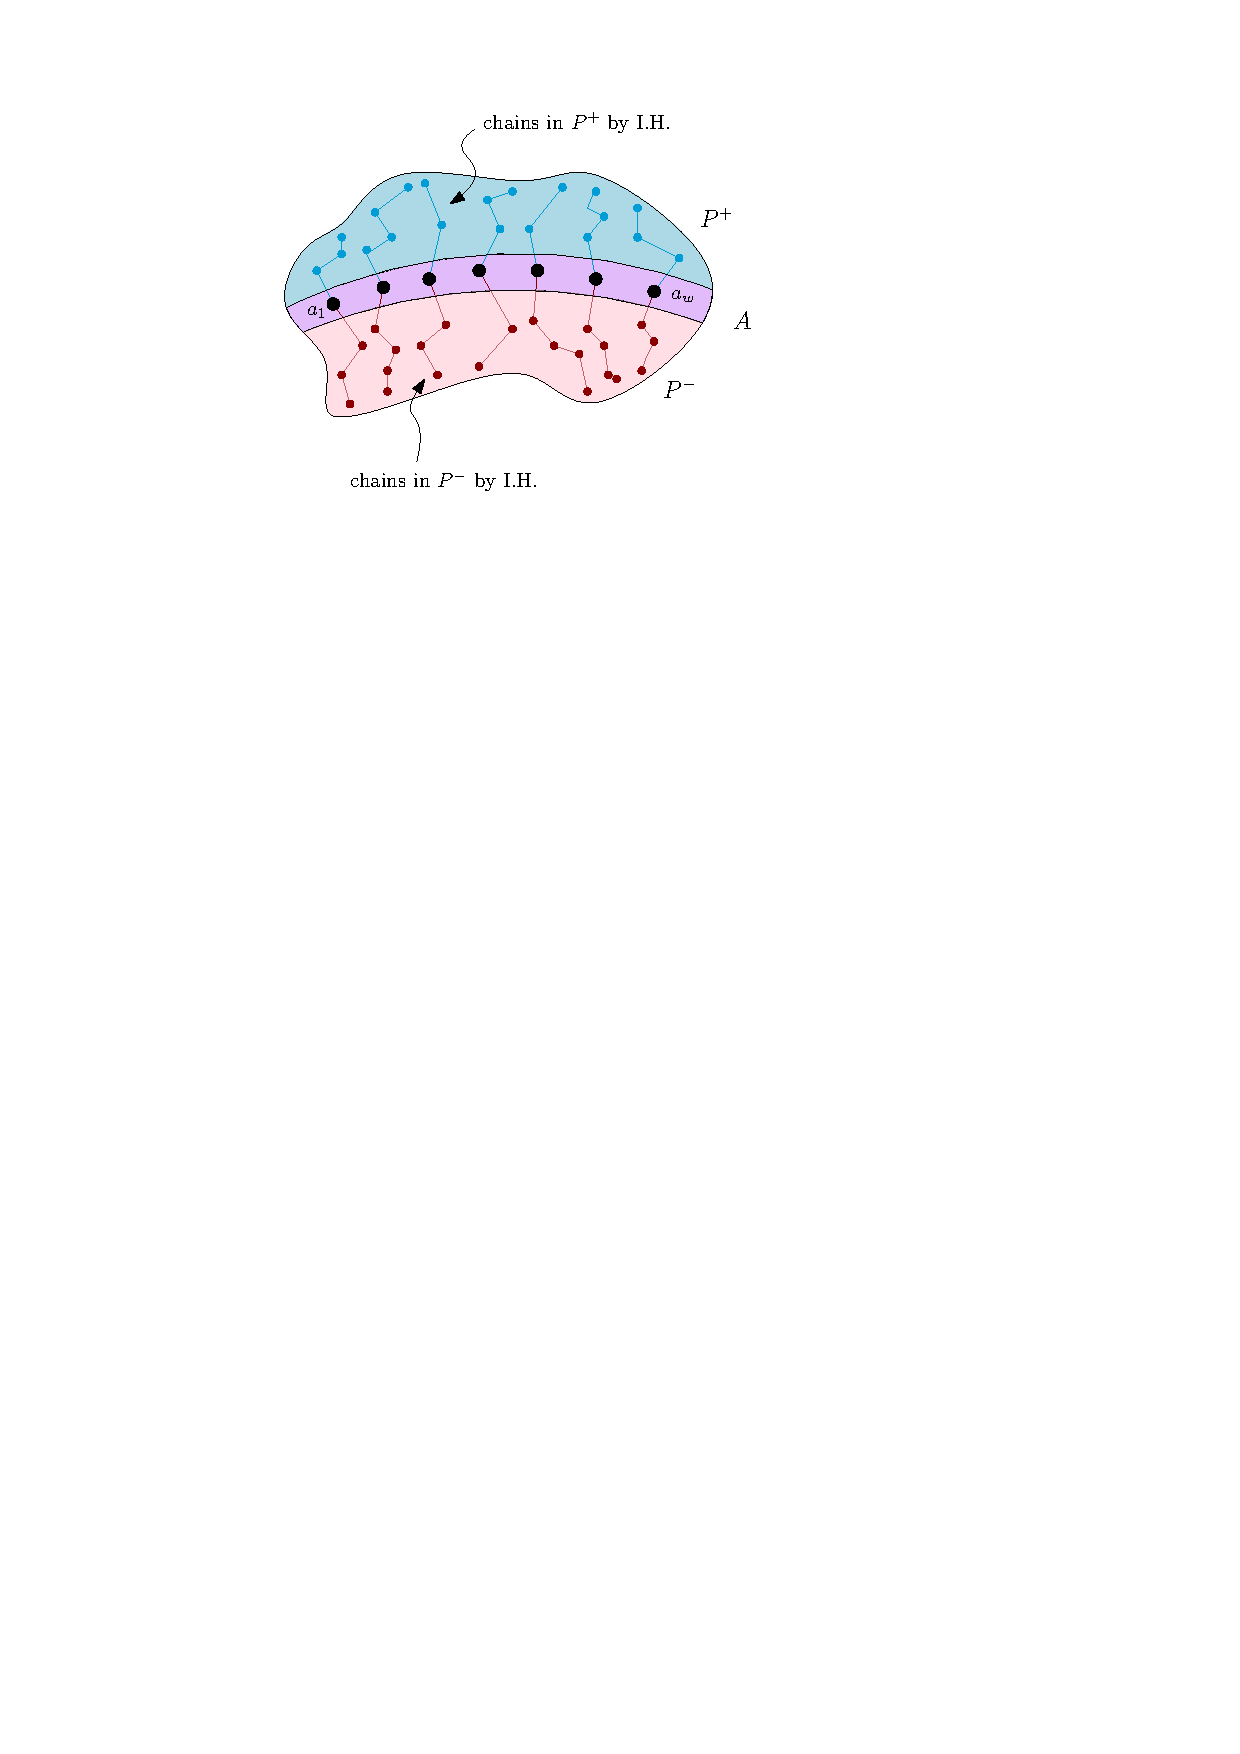
\includegraphics[width=0.4\linewidth]{figures/dilworth-proof-partition.pdf}
        \caption{We partition $P$ into $P^+$ and $P^-$ such that $P^+ \cap P^- = A$ and $P^+ \cup P^- = P$. Then, we take the $w$ chains in $P^+$ and concatenate with the $w$ chains in $P^-$ to form a set of $w$ disjoint chains in $P$.}
        \label{fig:dilworth-proof-partition}
    \end{figure}

    We note that
    \begin{enumerate}
        \item $P = P^- \cup P^+$. Otherwise, there would be an element $x \in P$ that is incomparable with every elements of $A$ and $A$ would not have been a max-size antichain.
        \item $P^- \cap P^+ = A$. Otherwise, there would exist $x,i,j$ such that $a_i <_{\mathbb{P}} x <_{\mathbb{P}} a_j$ so $A$ is not antichain.
        \item $x_h \not\in P^-$. Otherwise, $x <_{\mathbb{P}} a_i$ for some $i$ and the chain $C$ is not a maximal chain.
    \end{enumerate}

    By the third observation, $|P^-| < |P|$. Apply the inductive hypothesis, and we see that $P^-$ can be partitioned into $w$ chains $C^-_1,\ldots, C^-_w$. $a_i$ would be the \textbf{minimal element} in each $C^-_i$ because otherwise, $C^- \in P^- \cup P^+ \setminus A$, which contradicts the second observation. Using the same argument, we show that $P^+$ can be partitioned into $w$ chains $C^+_1,\ldots,C^+_w$ with $a_i$ as the minimal element of $C^+_i$.

    Now we construct the chains in $P$. Let $C_i = C^-_i \cup C^+_i$ so $P = \bigcup_{i=1}^w C_i$. From the second observation, it is clear that $C_i$ is a chain for $i = \{1,\ldots,w\}$.

    By induction, Dilworth's theorem holds for all posets.
\end{proof}

\subsection{Erd\"os-Szekeres}

\begin{theorem}[Erd\"os-Szekeres]
    Let $\{x_i \mid i \in [rs + 1]\}$ be a family of $rs + 1$ distinct real numbers. There is a strictly increasing subsequence of length $r+1$ or a strictly decreasing subsequence of length $s+1$.
\end{theorem}

Erd\"os-Szekeres's theorem can be proved using the Pigeonhole Principle. Here, we consider an alternative proof using Dilworth's theorem.

\begin{proof}
    Consider the poset $\mathbb{P} = (X,P)$ where
    $$
    X = \{ (i,x_i) \mid i \in [rs + 1]\}
    $$
    and $(i,x_i) \leq_{\mathbb{P}} (j,x_j)$ if and only if $i \leq j$ and $x_i \leq x_j$.

    If $\mathsf{height}(\mathbb{P}) \geq r+1$, we are done since a maximal chain contains strictly increasing subsequence $x_{n_k}$ of size at least $r+1$. 
    
    Hence, suppose $\mathsf{height}(\mathbb{P}) \leq r$. By Dilworth's theorem, there exists a partition of $P$ into $w$ chains $C_1,\ldots,C_w$. Note that $|C_i| \leq r$, so $w \geq s + 1$. Otherwise, we can cover $X$ of size $rs + 1$ with $\bigcup_{i=1}^w C_i$ which has at most $rs$ points, which is a contradiction.

    It follows that there is an antichain $A = \{(n_1,x_{n_1}),\ldots,(n_{r+1}, x_{n_{r+1}})\}$ where we may assume that $i < j$ implies $n_i < n_j$. By the way we defined $\mathbb{P}$, if $n_i < n_j$, then $x_{n_i} > x_{n_j}$ or else $A$ would not be an antichain. It follows then that $x_{n_i}$ is a decreasing subsequence of size at least $s+1$.
\end{proof}

\section{Linear Extensions}

\begin{definition}[Linear Extension]
    Let $\mathbb{P} = (X,P)$ be a poset. A linear extension of $\mathbb{P}$ is a linear (total) order $\mathbb{L} = (X,L)$ where $P \subseteq L$ (such that for all $a,b \in X$, $a \leq_{\mathbb{P}} b \iff a \leq_{\mathbb{L}} b$).
\end{definition}

Questions pertaining to extending posets to linear (total) orders relate to sorting algorithms. The following theorem states that every poset has a linear extension.

\begin{theorem}
    Let $\mathbb{P} = (X,P)$ be a poset. There is a linear extension $\mathbb{L} = (X,L)$ of $\mathbb{P}$.
\end{theorem}

\begin{proof}
    We prove this by recursively creating a sequence of extensions $\mathbb{P}_i = (X,P_i)$ of $\mathbb{P}$ starting from $\mathbb{P}$, and in the end we get a linear order.

    For some index $i$, we have a poset $\mathbb{P}_i$. If $\mathbb{P}_i$ is not a linear order, there must be two points $a,b \in X$ that are not $\mathbb{P}_i$-comparable. We construct $\mathbb{P}_{i+1}$ to be $(X,P_{i+1})$ where $P_{i+1}$ is
    $$
    P_{i+1} = P_i \cup \{ (a,b) \} \cup \{ (x,y) \in X^2 \mid x \leq_{\mathbb{P}_i} a \land b \leq_{\mathbb{P}_i} y \}.
    $$
    One can verify that $\mathbb{P}_{i+1}$ satisfies all the required properties of a poset, in particular, transitivity.

    We perform this process starting from the original poset $\mathbb{P}$ and eventually the process must half. Otherwise, we would have an infinite sequence of pairs $(a_i,b_i) \in X^2$ that are incomparable, contradicting that $X$ is finite.
\end{proof}

\end{document}